\documentclass[11pt]{article}

% ============================================================
% Milestone 2 -- Progress Report
% DIP Team Project -- Project 28
% Built from the official Section 6.2 template.
% ============================================================
\usepackage[margin=1in]{geometry}
\usepackage[T1]{fontenc}
\usepackage[utf8]{inputenc}
\usepackage{newtxtext,newtxmath}
\usepackage{microtype}
\usepackage{amsmath}
\usepackage{graphicx}
\usepackage{booktabs}
\usepackage[round]{natbib}
\usepackage{hyperref}
\hypersetup{
  colorlinks=true,
  linkcolor=blue!50!black,
  citecolor=blue!50!black,
  urlcolor=blue!50!black,
  pdftitle={Milestone 2 Progress Report: Building and Validating a Lightweight No-Reference Image-Quality Metric},
  pdfauthor={Novert Ahmed Fahim Abdelfattah, Farah Hossam Eldin Mahmoud, Mohamed Ahmed Fathy Abdelrazik}
}
\usepackage{enumitem}
\usepackage{xcolor}
\usepackage{caption}
\usepackage{array}
\usepackage{needspace}
\usepackage{float}
\usepackage{titlesec}
\usepackage{fancyhdr}

\captionsetup{font=small,labelfont=bf,skip=6pt}
\renewcommand{\arraystretch}{1.08}
\setlength{\textfloatsep}{10pt plus 2pt minus 2pt}
\setlength{\intextsep}{8pt plus 2pt minus 2pt}
\setlength{\abovecaptionskip}{4pt}
\setlength{\belowcaptionskip}{0pt}
\titleformat{\section}{\large\bfseries}{\thesection}{0.6em}{}
\titlespacing*{\section}{0pt}{2.2ex plus .4ex minus .2ex}{1ex}
\titleformat{\subsection}{\normalsize\bfseries}{\thesubsection}{0.5em}{}
\titlespacing*{\subsection}{0pt}{1.6ex plus .3ex minus .2ex}{0.6ex}

\pagestyle{fancy}
\fancyhf{}
\fancyhead[L]{\footnotesize CSE681 --- Project 28}
\fancyhead[R]{\footnotesize Milestone 2 --- Progress Report}
\fancyfoot[C]{\footnotesize \thepage}
\renewcommand{\headrulewidth}{0.4pt}
\fancypagestyle{plain}{%
  \fancyhf{}%
  \fancyfoot[C]{\footnotesize \thepage}%
  \renewcommand{\headrulewidth}{0pt}%
}

\setlength{\emergencystretch}{2em}
\renewcommand{\bibsection}{\section*{References}}
\renewcommand{\bibfont}{\footnotesize}
\setlength{\bibsep}{2pt plus 1pt}

\graphicspath{{figures/}}

\title{\LARGE Progress Report \\[4pt]
\large Building and Validating a Lightweight No-Reference Image-Quality Metric}
\author{
  Novert Ahmed Fahim Abdelfattah - 2501922 \\
  Farah Hossam Eldin Mahmoud - 2501897 \\
  Mohamed Ahmed Fathy Abdelrazik - 2400008
}
\date{Milestone 2 --- 17/11/2026 \\{} CSE681 --- Advanced Digital Image Processing}

\begin{document}
\maketitle

\begin{abstract}
No-reference image-quality assessment predicts the quality of a single distorted image
without a pristine reference. This report covers the second milestone. We reproduced the
M1 full-reference baselines on the held-out KADID-10k test split (LPIPS 0.808 SROCC,
PSNR 0.667, SSIM 0.627), built the training and evaluation code, and trained both compact
and foundation-encoder models. Our best model so far is a partially fine-tuned
SigLIP-B/16 at 384 px, using distortion and level auxiliary heads, a ranking loss, flip
TTA and KonIQ-10k as extra data. It reaches \textbf{0.9481 $\pm$ 0.0096 SROCC} over five
content folds and \textbf{0.7429 $\pm$ 0.0113} zero-shot on TID2013 with 93.4 M
parameters. The M1 minimum-viable deliverable is essentially met, although we had to
substitute the backbone (Section~\ref{sec:challenges}).
\end{abstract}

\section{Recap}
\label{sec:recap}

No-reference image-quality assessment is the part of the field that still works when the
clean image is gone. Images are compressed, resized, filtered and re-encoded before
anyone scores them, and PSNR, SSIM or LPIPS are usually unavailable because all three
need the reference. Our project trains a regressor from one distorted image to a human
quality label. We train and test on KADID-10k \citep{lin2019kadid} and use TID2013
\citep{ponomarenko2015tid2013} as a cross-dataset check.

KADID-10k contains 10,125 distorted images made from 81 reference contents, with 25
distortion types at five levels. Its MOS is given as DMOS in [1, 5], where higher is
better. TID2013 has 3,000 images from 25 references and 24 distortion types.
KonIQ-10k \citep{hosu2020koniq} adds 10,073 authentically distorted images and serves as
extra training data. The M1 baseline table used PSNR, SSIM and LPIPS
\citep{zhang2018lpips}. Our protocol splits by reference content rather than by distorted
image, and reports SROCC together with PLCC/RMSE after a four-parameter logistic fit.
All headline runs use seed 42.

\section{Implementation Status}
\label{sec:status}

The repository now holds a full experiment framework under \texttt{src/nriqa}. It covers
YAML configuration with inheritance, content-held-out and five-fold splits, training with
AMP, EMA and early stopping, prediction export, bootstrap confidence intervals, paired
significance tests, cross-dataset evaluation, ablations, hyper-parameter search, PyIQA
benchmarking and an inference-cost profiler. Each run saves its resolved configuration,
environment and git SHA, per-epoch metrics, predictions and a summary. The old M1 scripts
and tests are still in place and still produce the baseline table.

\subsection{Baseline Reproduction}
\label{sec:baseline}

Table~\ref{tab:baseline} reruns the M1 baseline on the 2,000-image test split, which holds
out 16 reference contents. LPIPS is a distance, so its raw correlation with DMOS is
negative. The table reports the magnitude, and the caption gives the sign convention. The
numbers match what the M1 pipeline produced, which tells us that the data pipeline, the
content split and the metric code are working as intended. Figure~\ref{fig:baselines}
shows the same correlations image by image.

\begin{table}[H]
\centering
\caption{M1 full-reference baselines on the content-held-out KADID-10k test split
(2,000 images). LPIPS is oriented so that higher is better; its raw SROCC is
$-0.808$.}
\label{tab:baseline}
\small
\begin{tabular}{@{}lccc@{}}
\toprule
\textbf{Metric} & \textbf{SROCC} & \textbf{PLCC} & \textbf{RMSE} \\
\midrule
PSNR  & 0.667 & 0.670 & 0.803 \\
SSIM  & 0.627 & 0.616 & 0.852 \\
LPIPS & 0.808 & 0.807 & 0.639 \\
\bottomrule
\end{tabular}
\end{table}

\begin{figure}[H]
\centering
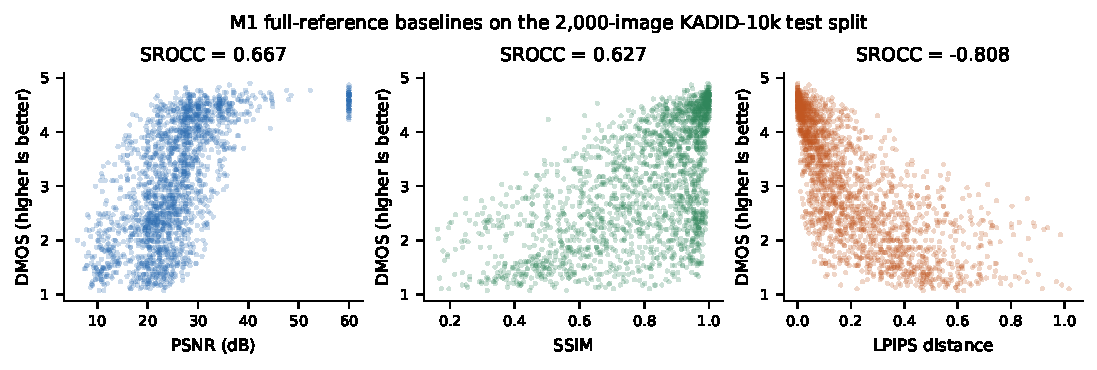
\includegraphics[width=\linewidth]{fig_m1_baselines.pdf}
\caption{M1 full-reference baselines on the 2,000-image KADID-10k test split. Each point
is one distorted image and the title gives the Spearman correlation with DMOS. LPIPS is
plotted as a distance, so its raw correlation is negative; Table~\ref{tab:baseline}
orients it.}
\label{fig:baselines}
\end{figure}

We also retrained published NR-IQA methods on matched splits. The best reproduction is
the B\_Gated+LoRA adapter recipe at 0.9424 content-held-out SROCC. MANIQA
\citep{yang2022maniqa}, TOPIQ \citep{chen2024topiq}, LIQE \citep{zhang2023liqe}, ARNIQA
\citep{agnolucci2024arniqa} and CLIP-IQA \citep{wang2023clipiqa} are part of the split
audit in Section~\ref{sec:results}. Every number there comes from our own runs, not from
the original papers.

\subsection{Proposed Method}
\label{sec:method}

The models fall into two groups.

\textbf{From-scratch statistical models.} MSOSNet (0.30 M parameters) combines a fixed
multi-scale MSCN pyramid with learned depthwise band-pass branches, orderless moment and
spatial-pyramid pooling, a 20-D colour descriptor, a coarse context branch and gated scale
fusion. WaveQNet (0.08 M) applies a fixed three-level Haar decomposition, computes
per-sub-band statistics and passes ten band/scale tokens through a small transformer. Both
lean on the natural-scene-statistics prior, which matters when only 57--64 reference
contents are available for training.

\textbf{Foundation encoders.} SigLIP-B/16 \citep{zhai2023siglip} is partially fine-tuned.
The patch embedding and the first eight of twelve ViT blocks stay frozen; the remaining
blocks, a regression head, distortion/level auxiliary heads and a pairwise ranking loss
are trained. We use 224 or 384 px crops, horizontal flips, no colour jitter, AdamW, cosine
scheduling, AMP and early stopping on validation SROCC. The headline model also trains on
KonIQ-10k, with the KADID distortion and level labels masked for KonIQ batches.
QStatFusion (94 M) gates SigLIP features against the MSOSNet statistical token, mainly to
improve cross-dataset robustness.

M1 proposed a frozen MobileNetV3-Large with a small MLP head. We implemented MobileNetV3
and the light-head pattern, but the compact model actually trained for M2 is
MobileNetV3-Small with full fine-tuning (0.721 SROCC). The foundation models go beyond the
M1 plan. We treat this as a deviation rather than presenting it as the original design;
Section~\ref{sec:challenges} gives the reasoning.

\section{Preliminary Results}
\label{sec:results}

Table~\ref{tab:models} compares the implemented models on the single content split we used
for quick iteration. Their capacities differ a lot, so the table is a diagnostic, and a
larger model is not automatically the better engineering choice. The five-fold result
appears separately in Table~\ref{tab:cv}.

\begin{table}[H]
\centering
\footnotesize
\caption{Single content split (57 train / 8 validation / 16 test references). TID2013 is
zero-shot for KADID-only models. QStatFusion and the compact models use this split; the
best five-fold result is in Table~\ref{tab:cv}.}
\label{tab:models}
\setlength{\tabcolsep}{3pt}
\begin{tabular}{@{}lrrrr@{}}
\toprule
\textbf{Method} & \textbf{Params} & \textbf{KADID SROCC} & \textbf{KADID PLCC} & \textbf{TID2013 SROCC} \\
\midrule
WaveQNet (from scratch)        & 0.08 M  & 0.496 & 0.547 & 0.234 \\
MSOSNet (from scratch)         & 0.30 M  & 0.721 & 0.730 & 0.483 \\
MobileNetV3-Small (fine-tuned) & 1.52 M  & 0.721 & 0.732 & 0.632 \\
ResNet-18 (fine-tuned)         & 11.2 M  & 0.769 & 0.779 & 0.678 \\
SigLIP-B/16 224 + aux/rank/TTA & 93.1 M  & 0.897 & 0.907 & 0.726 \\
QStatFusion 224                & 93.8 M  & 0.889 & 0.897 & \textbf{0.753} \\
\bottomrule
\end{tabular}
\end{table}

\begin{figure}[H]
\centering
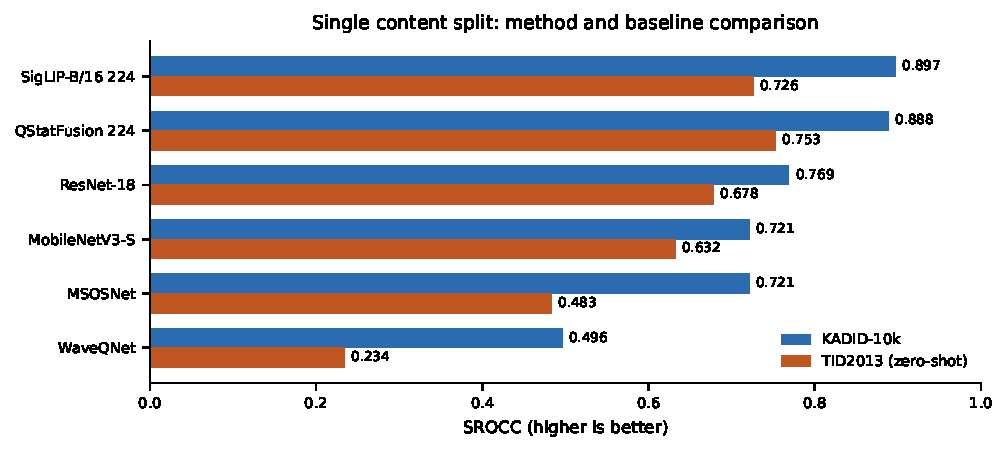
\includegraphics[width=0.92\linewidth]{fig_model_comparison.pdf}
\caption{Single-split comparison of the implemented models. The from-scratch models
(0.08--0.30 M) sit far below the foundation encoders. QStatFusion gives up a little KADID
accuracy for the best TID2013 result on this split.}
\label{fig:models}
\end{figure}

The split protocol turned out to matter more than any single model result. Published
methods retrained on matched random and content-held-out splits score much higher on
random splits, because different distorted versions of the same reference end up in both
train and test (Figure~\ref{fig:split}). B\_Gated+LoRA moves from 0.9424 to 0.9731, our
model from 0.9416 to 0.9670, and MANIQA from 0.8830 to 0.9704. Under the content protocol
the top three methods are statistically tied. The fair reading is that a 93.4 M model
matches much larger foundation probes; we do not claim to beat them.

\begin{figure}[H]
\centering
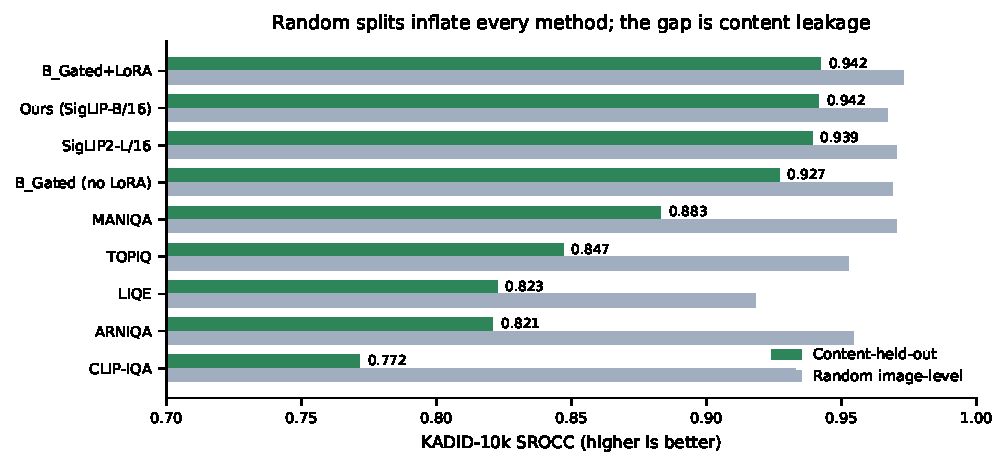
\includegraphics[width=0.92\linewidth]{fig_split_audit.pdf}
\caption{Random versus content-held-out KADID-10k SROCC, with every method retrained under
matched splits. The gap is content leakage: a model looks much stronger when different
distorted versions of the same reference appear in both train and test.}
\label{fig:split}
\end{figure}

Figure~\ref{fig:distortion} shows the 384 px model by distortion family. Colour saturation
(0.941), block-wise distortions (0.934), Gaussian blur (0.933) and Gaussian noise (0.927)
are handled well. Hue shift (0.476), sparse sampling (0.496), multiplicative noise (0.499)
and quantisation (0.557) are much weaker. Those failures explain the colour-aware and
frequency-aware work planned for M3.

\begin{figure}[H]
\centering
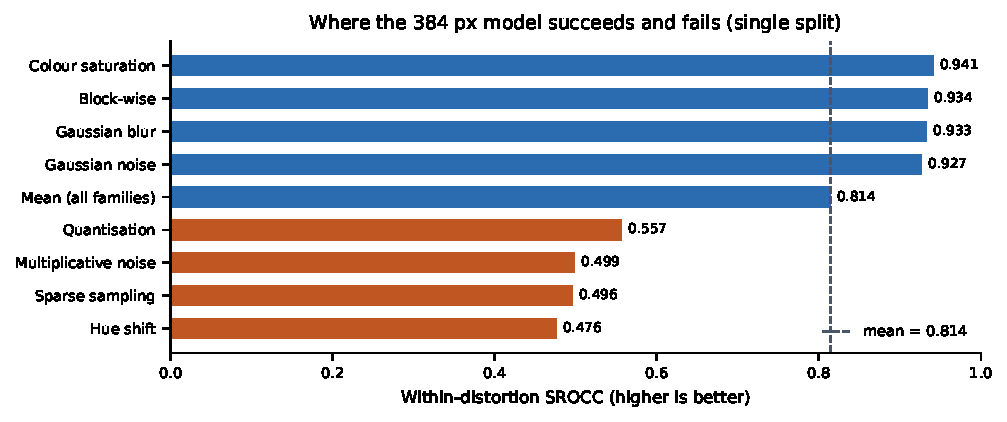
\includegraphics[width=0.92\linewidth]{fig_per_distortion.pdf}
\caption{Within-distortion SROCC for the 384 px single-split model. The dashed line marks
the mean over families (0.814). Hue shift and sparse sampling remain the clearest
failures.}
\label{fig:distortion}
\end{figure}

\begin{table}[H]
\centering
\small
\caption{Five-fold content cross-validation on KADID-10k. Each fold holds out 16 reference
contents. TID2013 is evaluated zero-shot from the KADID-trained checkpoint.}
\label{tab:cv}
\setlength{\tabcolsep}{3pt}
\begin{tabular}{@{}lrrrr@{}}
\toprule
\textbf{Method} & \textbf{Params} & \textbf{KADID SROCC} & \textbf{KADID PLCC} & \textbf{TID2013 SROCC} \\
\midrule
SigLIP-B/16 384, KADID + KonIQ & 93.4 M  & \textbf{0.9481 $\pm$ 0.0096} & \textbf{0.9524} & \textbf{0.7429 $\pm$ 0.0113} \\
SigLIP-L/16 384 + aux/rank/TTA & 316.6 M & 0.9481 $\pm$ 0.0074 & 0.9526 & 0.7232 $\pm$ 0.0205 \\
SigLIP-B/16 384 + aux/rank/TTA & 93.4 M  & 0.9393 $\pm$ 0.0149 & 0.9441 & 0.7166 $\pm$ 0.0123 \\
\bottomrule
\end{tabular}
\end{table}

\section{Challenges \& Deviations from the M1 Plan}
\label{sec:challenges}

\textbf{The backbone changed.} M1 specified a frozen MobileNetV3-Large with an MLP head.
We trained a fully fine-tuned MobileNetV3-Small instead, and the main line later moved to
a partially fine-tuned SigLIP-B/16. The reason is simple: compact and from-scratch models
stop around 0.72 SROCC with 57--64 training contents, while frozen foundation features
carry much more quality information. We kept the low-parameter, light-head idea and
changed the encoder. The code can build MobileNetV3-Large and has a \texttt{freeze}
switch, so the exact M1 MVP is a short run. We would rather list it as pending than report
a number we did not produce.

\textbf{Random splits were misleading.} The first pilots used the usual image-level split
and gave correlations near 0.97. A content-level check showed that most of that gain came
from content leakage. We moved every headline number to content-held-out or five-fold
splits and added the audit to the repository. This departs from much of the NR-IQA
literature, deliberately.

\textbf{Full fine-tuning overfits.} Unfreezing all 93 M parameters on 57 training contents
peaks early and then degrades. Partial fine-tuning was better every time we tried it, and
the compact CNNs showed the same pattern. Partial fine-tuning is therefore the default;
full fine-tuning is only an ablation.

\textbf{Published methods were unstable.} LIQE and MANIQA collapsed on the small content
split until we switched to native cross-entropy or soft-label objectives. The split audit
records the recipe that worked for each method. It also makes clear that a random-split
ranking tells us little about the content ranking.

\textbf{Resolution and data.} Higher resolution helps within KADID but can hurt
cross-dataset generalisation, and training on KonIQ creates a large dependency on authentic
data. We report both sides instead of keeping only the favourable number.

\section{Updated Work Breakdown \& MVP Status}
\label{sec:workbreakdown}

The M1 minimum-viable deliverable was a trained NR-IQA model with a valid comparison
against the full-reference baselines. We have that: a trained compact baseline and a
stronger foundation model, both evaluated on the same content-held-out split as PSNR, SSIM
and LPIPS. One caveat remains. The exact M1 configuration, a frozen MobileNetV3-Large, is
not the configuration we ran, and Section~\ref{sec:challenges} explains why. We describe
the MVP as \emph{met in all but one respect, with a documented backbone substitution}; the
literal M1 recipe has not been executed.

\begin{table}[H]
\centering
\small
\caption{Updated milestone allocation. The M2 column lists what was completed; the M3
column is the plan for Weeks 7--9.}
\label{tab:tasks}
\begin{tabular}{@{}>{\raggedright\arraybackslash}p{0.12\linewidth}>{\raggedright\arraybackslash}p{0.26\linewidth}>{\raggedright\arraybackslash}p{0.26\linewidth}>{\raggedright\arraybackslash}p{0.26\linewidth}@{}}
\toprule
\textbf{Milestone} & \textbf{Student A} & \textbf{Student B} & \textbf{Student C} \\
\midrule
M2 (Wk 6) -- completed &
Dataset/split pipeline; baseline reproduction; split audit &
Model and training code; compact and foundation checkpoints; ablations &
Evaluation harness; CV/bootstrap tables; figures and this report \\
M3 (Wk 9) -- planned &
Final baselines; TID2013/KonIQ pipeline; reproducibility check &
Final model and ablations; efficiency measurements &
Cross-dataset table; demo; final report figures \\
\bottomrule
\end{tabular}
\end{table}

\section{Next Steps}
\label{sec:next}

\begin{enumerate}[leftmargin=*]
  \item Run the literal frozen MobileNetV3-Large MVP once, as a completeness check, or
        state the substitution in the final report.
  \item Freeze the M2 checkpoint, publish its path and record the resolved configuration
        used for the headline model.
  \item Add a dependency lock file and align it with the environment that produced the
        reported runs.
  \item Extend the per-distortion analysis with qualitative examples and per-image errors
        for M3.
  \item Finish the M3 ablation and cross-dataset tables, then package the demo and final
        report.
\end{enumerate}

\needspace{9\baselineskip}
\section*{AI-Tool Usage Disclosure}
AI tools helped with code scaffolding, debugging, literature search and \LaTeX{} editing.
Research planning, study design, experimental runs and all reported numbers were carried
out and checked by the team.

\bibliographystyle{unsrtnat}
\bibliography{references}

\end{document}
